\label{chapt:intro}

It is hard to imagine that there was ever a period of time where the need for instant communication was not a daily need. Constant access to cellular service and other telecommunication, regardless of location, is no longer an option but a requirement. Up nearly 13\% from last year, it is said that US consumers are checking their mobile devices at a remarkable rate of 9 billion times per day \cite{deloittestat}.\\

It is numbers like these that have inspired \Company to begin research and development on a new way to provide this service more effectively. Altaeros is determined to develop the worlds first fully autonomous commercial aerostat's as a replacement to the conventional cellular tower. The latest version of their aerostat is seen below in Figure~\ref{fig:1_companypic}.

\begin{figure}[H]
	\centering
	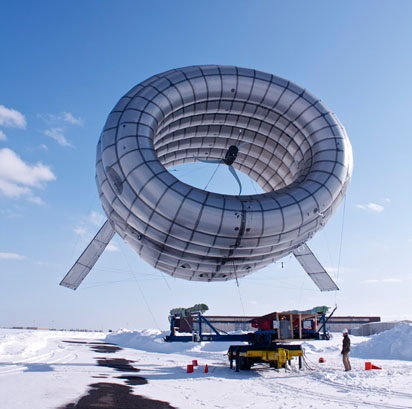
\includegraphics[scale=0.4]{1_companypic}
	\caption[Overview of Altaeros' aerostat.]{Overview of Altaeros' aerostat.\protect\cite{companypicweb}}
	\label{fig:1_companypic}
\end{figure}

From the above figure, the grounded tether management system (TMS) can be observed. This report will focus on the structural design of one of this system's components.

\section{Background} 

A key TMS component responsible for full control of the aerostat is the winch system. An overview of similar system used by Altaeros is shown below in Figure~\ref{fig:1_winch}.
\begin{figure}[H]
	\centering
	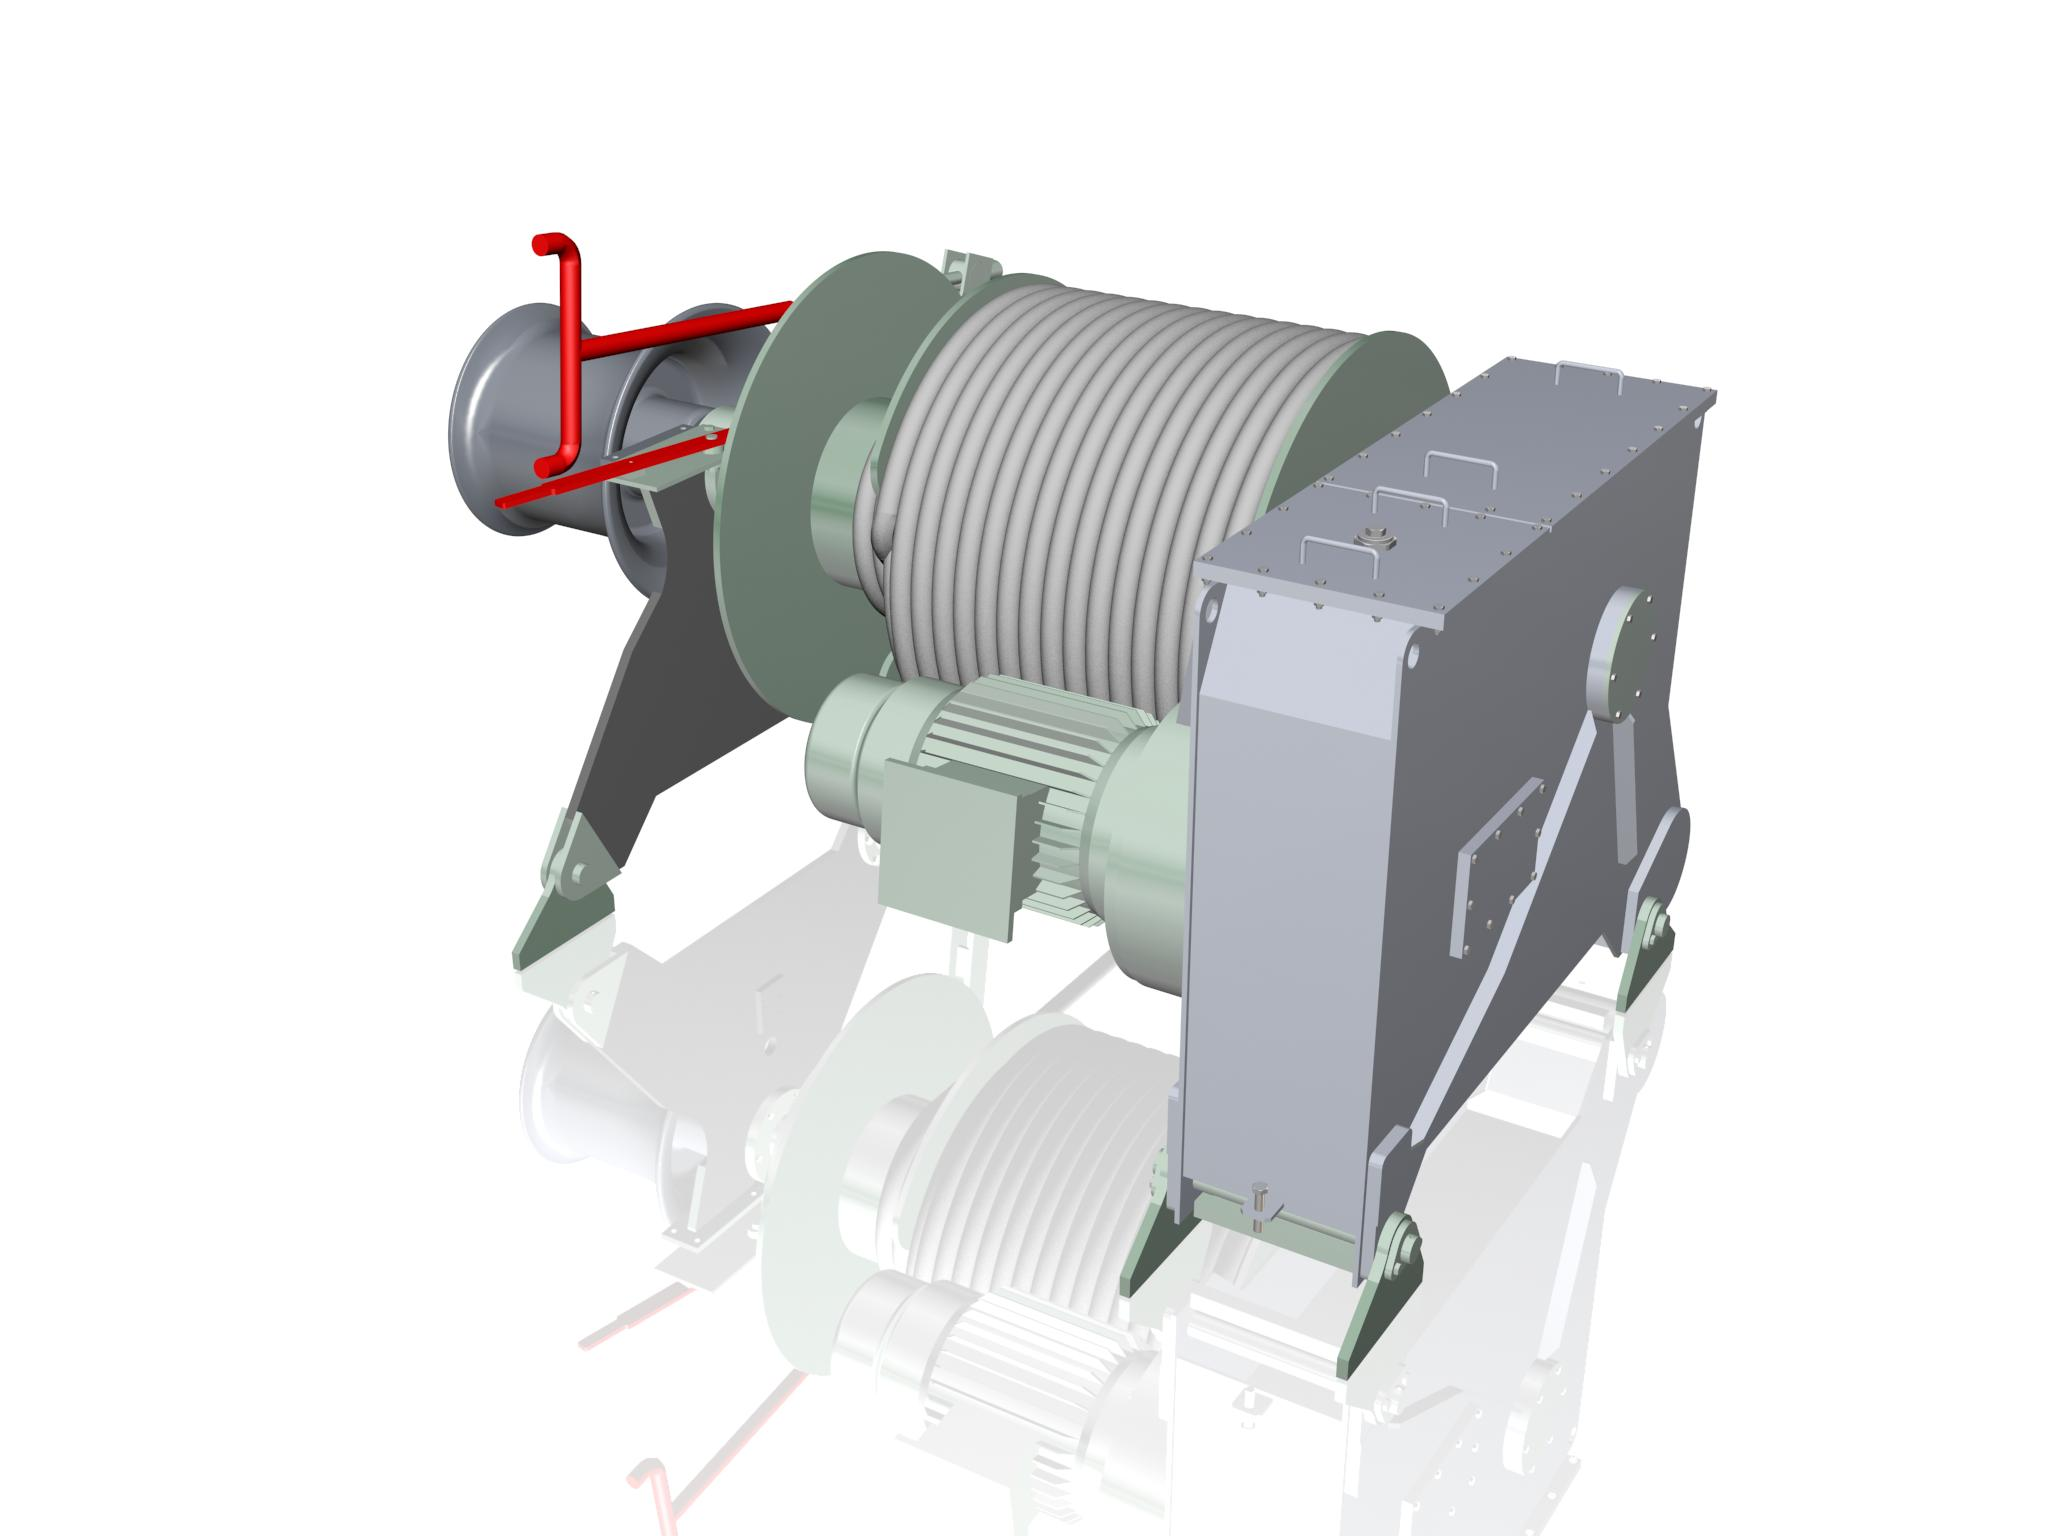
\includegraphics[scale=0.2]{1_winch}
	\caption[Example of a common winch system.]{Example of a common winch system.\protect\cite{winchpic}}
	\label{fig:1_winch}
\end{figure}

From above, a tether or cable is wound on the winch drum. As required, this tether is reeled in or out to control the altitude of the aerostat.\\

In the past, these winch systems were purchased from a third party vendor. After much though, it was deemed feasible that Altaeros could manufacture a more custom, cheaper and efficient winch system. To assure that the system is capable of handling the large aerodynamic loads translated by the tether, a complete structural analysis must be completed.

\section{Purpose}

The purpose of this report is to perform a structural analysis to assure that the winch drum assembly is capable of handling the maximum tether loads. This analysis will focus on sizing the thickness of both the drum barrel and flanges.\\

An overview of the winch's drum assembly is shown in the 3D computer aided design (CAD) model \cite{INVENTOR} in Figure~\ref{fig:1_drum}.
\begin{figure}[H]
	\centering
	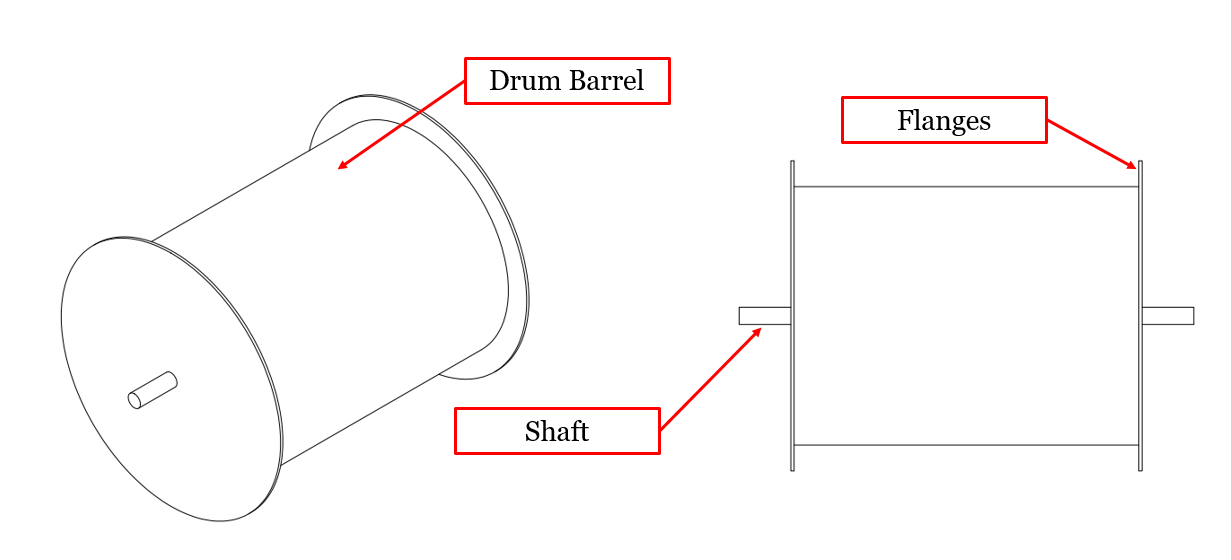
\includegraphics[scale=0.4]{1_drum}
	\caption{Drum assembly CAD model.}
	\label{fig:1_drum}
\end{figure}

It is important to realize that most of loading from the tether will be translated as pressure onto the barrel. This loading scenario will be investigated to properly size the winch barrel thickness.

\section{Scope}

In the following sections of this report, the relevant assembly parameters, loads and material properties will be presented. A preliminary analysis will be completed to investigate how tether tension translates to external pressure. Furthermore, existing codes and standards will be explored to serve as a benchmark. From this, a more advanced analytical approach will be studied. These results will then be compared and validated through a series finite element analysis (FEA) runs. The report will conclude with a summary of all results as  well as relevant discussion, conclusions and recommendations points. Please note that most of this report will utilize imperial units however, relevant findings will be converted to metric equivalents.